%! TEX root = ./main.tex

\section{Planning}
\begin{itemize}
    \ides{Completeness:} A robot system is complete iff for all possible problems, when a solution trajectory exists, the system will find it
\end{itemize}
\subsection{Path Planning}
\begin{itemize}
    \ides{Problem:} Find path in the physical space from the initial position to the goal position avoiding obstacles
    \ides{Workspace:} Physical area where the robot moves
    \ides{Configuration Space $C$:} $k$-dimensional space representing all configurations (position, rotations etc.) of a robot:
        \begin{itemize*}
            \item Occupied areas $O$
            \item Free areas $F = C \setminus O$
        \end{itemize*}
\end{itemize}

\subsubsection{Graph Search}
\begin{itemize}
    \ides{Idea:} Search path in connectivity graph of free space
    \item Consists of two steps
    \item[1)] \textbf{Graph Construction}
        \begin{itemize}
            \ides{Visibility Graph}
                \begin{itemize}
                    \item
                        \begin{itemize}
                            \item Polygonal configuration space
                            \item Robot is a point $\implies$ enlarge obstacles
                            \item Connect corners which ``see'' each other
                        \end{itemize}
                    \ipro Gives shortest path
                    \icon Complexity depends on number of obstacles
                    \icon Path is close to obstacles
                    \icon Does not consider robot motion constraints
                \end{itemize}
            \ides{Voroni Diagram}
                \begin{itemize}
                    \item
                        \begin{itemize}
                            \item For each point in free space compute the distance to the nearest obstacle
                            \item Points which are equidistant to two obstacles for edges
                        \end{itemize}
                    \ipro Maximizes distance to obstacles
                    \ipro Can do the process in reverse. Robot in unknown environment creates diagram by moving on unknown veroni edges
                    \icon Not optimal
                    \icon Does not consider robot motion constraints
                \end{itemize}
            \ides{Exact Cell Decomposition}
                \begin{itemize}
                    \item
                        \begin{itemize}
                            \item Draw lines according to obstacle geometry
                            \item Each filed is in either $F$ or $O$
                            \item Create connectivity graph from cells in $F$
                        \end{itemize}
                    \item Assumes: precise position in $F$ does not matter
                        \icon Complexity depends on number and complexity of obstacles
                \end{itemize}
            \ides{Approximate Cell Decomposition}
                \begin{itemize}
                    \item
                        \begin{itemize}
                            \item Put grid over map
                            \item Each cell is either in $O$ or $F$
                            \item Create connectivity graph from cells in $F$
                        \end{itemize}
                        \ides{Fixed-Size:} Grid has fixed size
                        \ides{Variable-Size:} Recursively split partially occupied cells into $4$ new cells
                        \icon Loss of narrow passages
                \end{itemize}
            \ides{Lattice Graph}
                \begin{itemize}
                    \item
                        \begin{itemize}
                            \item Overlay space with custom edges/curves
                            \item Each cell is either in $O$ or $F$
                            \item Create connectivity graph from cells in $F$
                        \end{itemize}
                    \item Cell decomposition is a special case of it
                    \ipro Great freedom
                \end{itemize}
        \end{itemize}
    \item[2)] \textbf{Graph Search}
        \begin{itemize}
            \item Expected cost from start to goal via node $n$: $f(n) = \underbrace{g(n)}_{\text{cost so far}} + \epsilon \underbrace{h(n)}_{\substack{\text{cost to go} \\ \text{heuristic}}}$
            \ides{Breath-First Search (BFS)}
                \begin{itemize}
                    \item Nodes expanded according to FIFO queue and closed list
                    \item Solution is optimal for uniform edge cost
                    \item $\bigO(|V| + |E|)$
                    \ipro First solution found is optional
                    \item Greedy backtracking of solution
                    \ides{BF(Graph G, Node Start, Node Goal)}
                        \begin{algorithmic}
                            \STATE FIFO.push(Start)
                            \WHILE{FIFO not empty}
                                \STATE Node current $\leftarrow$ FIFO.pop()
                                \IF{current $==$ Goal}
                                    \RETURN SUCCESS
                                \ENDIF
                                \STATE visited.push(current)
                                \STATE Nodes next = getNeighbours(current)
                                \FORALL{next $\notin$ visited}
                                    \STATE FIFO.push(next)
                                \ENDFOR
                            \ENDWHILE
                            \RETURN FAILURE
                        \end{algorithmic}
                \end{itemize}
            \ides{Depth-First Search (DFS)}
                \begin{itemize}
                    \item Nodes expanded according to LIFO queue and closed list
                    \ipro Better space complexity
                    \item $\bigO(|V| + |E|)$
                    \icon First solution found may not be optional
                    \item Greedy backtracking of solution
                    \ides{DF:} Same as BF but using LIFO
                \end{itemize}
            \ides{Dijkstra's Algorithm}
                \begin{itemize}
                    \item Nodes expanded according to Min-Heap (on $g(n)$) and closed list
                    \item Positive edge cost
                    \item $\bigO(|V| \log(|V|) + |E|)$
                    \item Often computed from the goal position to get all distances to the goal
                    \ipro First solution found is optional
                    \item Greedy backtracking of solution
                    \ides{Dijkstra(Graph G, Node Start, Node Goal)}
                        \begin{algorithmic}
                            \STATE MIN-HEAP.push(Start)
                            \WHILE{MIN-HEAP not empty}
                                \STATE Node current $\leftarrow$ MIN-HEAP.pop()
                                \IF{current $==$ Goal}
                                    \RETURN SUCCESS
                                \ENDIF
                                \STATE visited.push(current)
                                \STATE Nodes next = getNeighbours(current)
                                \FORALL{next $\notin$ visited}
                                    \STATE MIN-HEAP.push(next)
                                \ENDFOR
                            \ENDWHILE
                            \RETURN FAILURE
                        \end{algorithmic}
                \end{itemize}
            \ides{$\mathbf{A^*}$}
                \begin{itemize}
                    \item Nodes expanded according to Min-Heap (on $f(n)$) and closed list
                    \item Heuristic function guides search
                        \begin{itemize}
                            \item Must underestimate the distance
                            \item Often $h(n) =$ Distance from $n$ to goal
                        \end{itemize}
                    \item Positive edge cost
                    \item Good for single source shortest path
                    \item Runtime depends on chosen $h(n)$
                    \ipro First solution found is optional
                    \ipro Very efficient if we are ok finding a suboptimal solution
                        \begin{itemize}
                            \item Done if $\epsilon > 1$
                        \end{itemize}
                    \item Greedy backtracking of solution
                    \ides{A-Star(Graph G, Heur H, Node Start, Node Goal)}
                        \begin{algorithmic}
                            \STATE HEUR-MIN-HEAP.push(Start)
                            \WHILE{HEUR-MIN-HEAP not empty}
                                \STATE Node current $\leftarrow$ HEUR-MIN-HEAP.pop()
                                \IF{current $==$ Goal}
                                    \RETURN SUCCESS
                                \ENDIF
                                \STATE visited.push(current)
                                \STATE Nodes next = getNeighbours(current)
                                \FORALL{next $\notin$ visited}
                                    \STATE HEUR-MIN-HEAP.push(next)
                                \ENDFOR
                            \ENDWHILE
                            \RETURN FAILURE
                        \end{algorithmic}
                \end{itemize}
            \ides{Rapidly Exploring Random Trees (RRTs)}
                \begin{itemize}
                    \item Grows randomized tree
                    \item Selects random points and connects it to closest point of the tree using a new branch
                    \item Most likely returns suboptimal solution
                    \item Probabilistically complete
                    \ides{RRT(Node Start, Node Goal, System Sys, Environment Env)}
                        \begin{algorithmic}
                            \STATE Graph.init(Start)
                            \WHILE{Graph.size() $\le$ threshold}
                                \STATE Node rand = random()
                                \STATE Node near = Graph.nearest(rand)
                                \STATE \textbf{try}
                                \STATE $\quad$ Node new = Sys.propagate(near, rand)
                                \STATE $\quad$ Graph.addNode(new)
                                \STATE $\quad$ Graph.addEdge(near, new)
                                \STATE \textbf{end try}
                            \ENDWHILE
                            \RETURN FAILURE
                        \end{algorithmic}
                \end{itemize}
        \end{itemize}
\end{itemize}

\subsubsection{Potential Field Planning}
\begin{itemize}
    \ides{Idea:} Robot follows gradient of potential field
    \item Global
    \item Implicit incorporation of basic system models
    \ides{Local Potential Fields}
        \begin{itemize}
            \ides{Potential Field:} $U(q) = \underbrace{U_{\text{att}}(q)}_{\text{attractive}} + \underbrace{U_{\text{rep}}(q)}_{\text{repulsive}}$
            \item $U_{\text{att}}(q) = \frac{1}{2} k_{\text{att}} (q - q_{\text{goal}})^2$
            \item $U_{\text{rep}}(q) =
\begin{cases}
    \frac{1}{2} k_{\text{rep}}(\frac{1}{\rho(q)} - \frac{1}{\rho_{\text{lim}}})^2 & \text{if } \rho(q) \ge \rho_{\text{lin}}\\
    0 & \text{otherwise}
\end{cases}$
            \item
                \begin{itemize*}
                    \ides{$\mathbf{\rho(q)}$:} Min distance between $q$ and the closest obstacle
                    \ides{$\mathbf{\rho_{\text{lim}}}$:} Distance of influence of obstacle
                    \ides{$\mathbf{k_{\text{att/rep}}}$:} Scaling factor
                \end{itemize*}
            \item Robot follows force $F(q) = -\bigtriangledown U(q)$
            \icon May get stuck in local minima
            \icon No incorporation of robot's dynamic constraints
        \end{itemize}
    \ides{Harmonic Potential Fields}
        \begin{itemize}
            \item Robots follows solution of Laplace Equation $\triangle U = \sum \frac{\partial^2 U}{\partial^2 q_i} = 0$
            \item Boundary is specified according to:
                \begin{itemize}
                    \ides{Neumann:}
                        \begin{itemize*}
                            \item Equidistant lines parallel to the obstacles
                            \icon Potentially small distance to the obstacle
                            \item $\frac{\partial U(q)}{\partial q} = g(q) = 0$
                        \end{itemize*}
                    \ides{Dirchlet:}
                        \begin{itemize*}
                            \item Obstacle boundaries have constant high potential
                            \item Goal has constant low potential
                            \item Close to obstacles, robot moves perpendicularly away from obstacle
                            \item $U(q) = f(q) = \text{const}$
                            \ipro Safe paths
                            \icon Long paths
                        \end{itemize*}
                \end{itemize}
            \ipro Absence of local minima
            \item Solved via discretization of the workspace into cells
            \item Euler approximation: $\bigtriangledown U(q)_i \approx \frac{U(q + \delta e_i) - U(q)}{\delta}$
            \item Iterative method: $U^{k+1}(q) = \frac{1}{2n} \sum_{i=1}^{n} (U^k(q + \delta e_i) + U^k(q - \delta e_i))$\\
                \begin{itemize*}
                    \ides{$\mathbf{n}$:} \# dimensions
                    \ides{$\mathbf{e_i}$:} unit vector
                \end{itemize*}
            \item Steps from iteration $i$ to $i+1$
                \begin{itemize}
                    \item[1)] Initialize cell values
                        \begin{itemize}
                            \ides{Dirchlet:} Set obstacles to $1$ and goal and all other cells to $0$
                        \end{itemize}
                    \item[2)] Update all cells except goal and obstacles
                        \begin{itemize}
                            \item[a)] Add up values of $4$ neighbouring cells
                            \item[b)] Scale sum by $2n$
                            \item[c)] Update cell values
                        \end{itemize}
                    \item[3)] Repeat 2 till convergence
                    \item[4)] Backtrack solution
                \end{itemize}
        \end{itemize}
\end{itemize}

\subsection{Obstacle Avoidance}
\begin{itemize}
    \item Function of current on optionally past sensor readings, its current and goal location
    \icon Prone to local minima
    \ipro Incorporate system model
    \ides{Dynamic Window Approach (DWA)}
        \begin{minipage}[b]{0.5\linewidth}
            \raggedright
            \begin{itemize}
                \item Assume: robot moves on circular arcs $(\nu, \omega)$
                \ides{Obstacle space $\mathbf{V_o}$:} Transformation of obstacles from workspace to input space
            \end{itemize}
        \end{minipage}
        \begin{minipage}[b]{0.45\linewidth}
            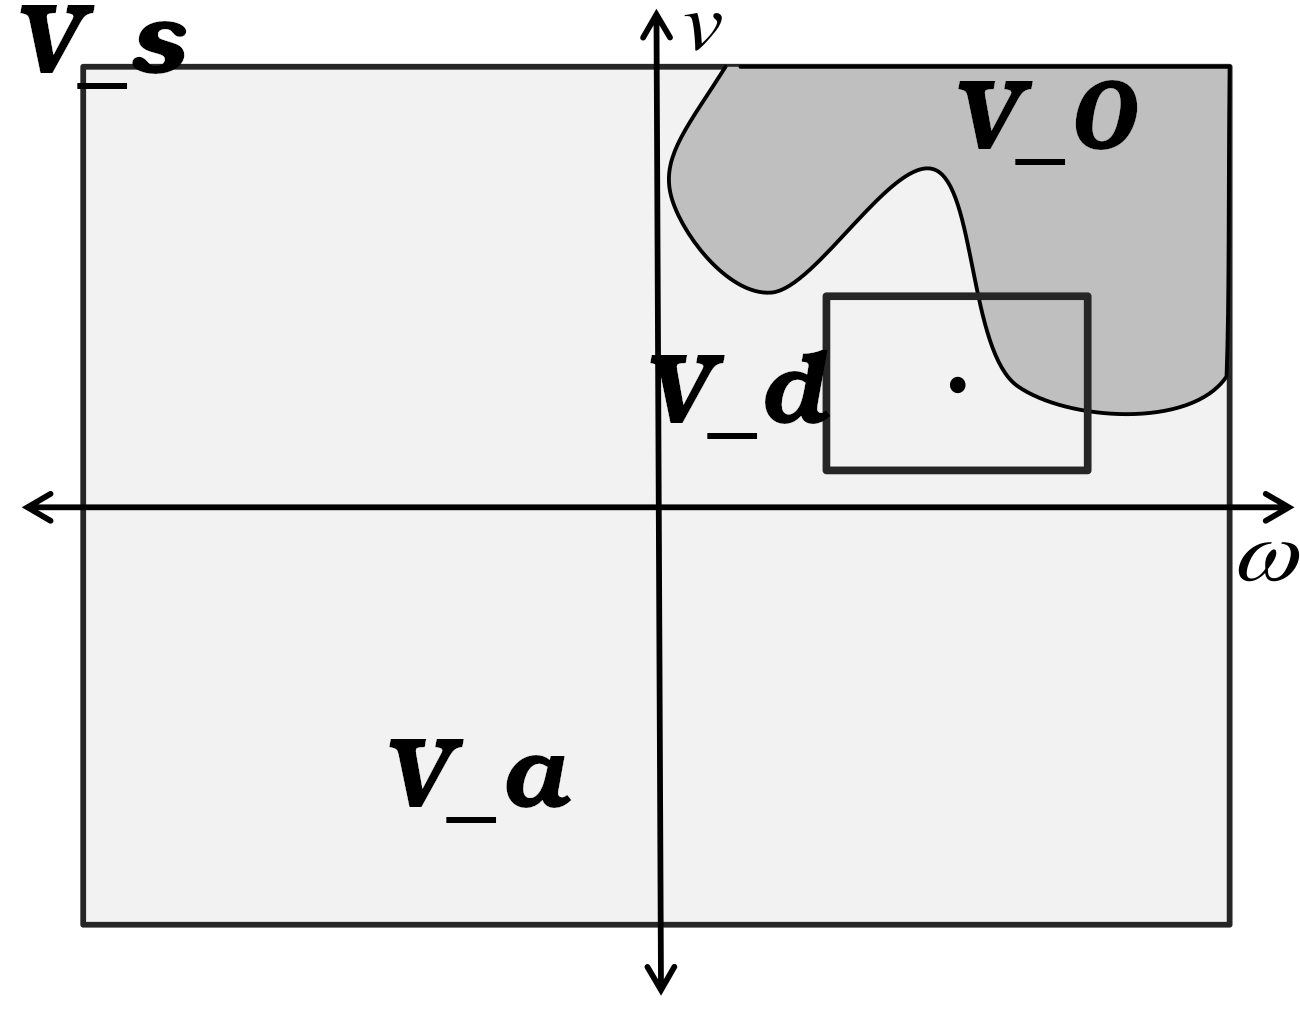
\includegraphics[width=0.97\linewidth]{./Figures/06_DWA.png}
        \end{minipage}
        \begin{itemize}
            \ides{Admissible space $\mathbf{V_a}$:} complement of $V_o$
            \ides{Static Window $\mathbf{V_s}$:} Configuration which are allowed by robot limits
            \ides{Dynamic Window $\mathbf{V_d}$:} Configuration which can be reached in one step
                \begin{itemize}
                    \item Centred around the current configuration
                \end{itemize}
            \ides{New configuration $\mathbf{V_r}$} $= V_a \cap V_s \cap V_d$
                \begin{itemize}
                    \item Selected which maximizes some objective function containing heading, distance to goal and velocity
                \end{itemize}
            \icon Not safe when obstacles are dynamic
        \end{itemize}
    \ides{Velocity Obstacles (VO)}
        \begin{minipage}[b]{0.5\linewidth}
            \raggedright
            \begin{itemize}
                \item Assume:
                    \begin{itemize*}
                        \item Robot moves on piece-wise linear curves
                        \item Robot is omnidirectional
                        \item Robot and obstacles are circular
                        \item Obstacles move at constant speed
                    \end{itemize*}
                \item Collision of robot and obstacle if $\lVert p_\text{RO} + \nu_R t \rVert < r_\text{R} + r_\text{O}$
            \end{itemize}
        \end{minipage}
        \begin{minipage}[b]{0.45\linewidth}
            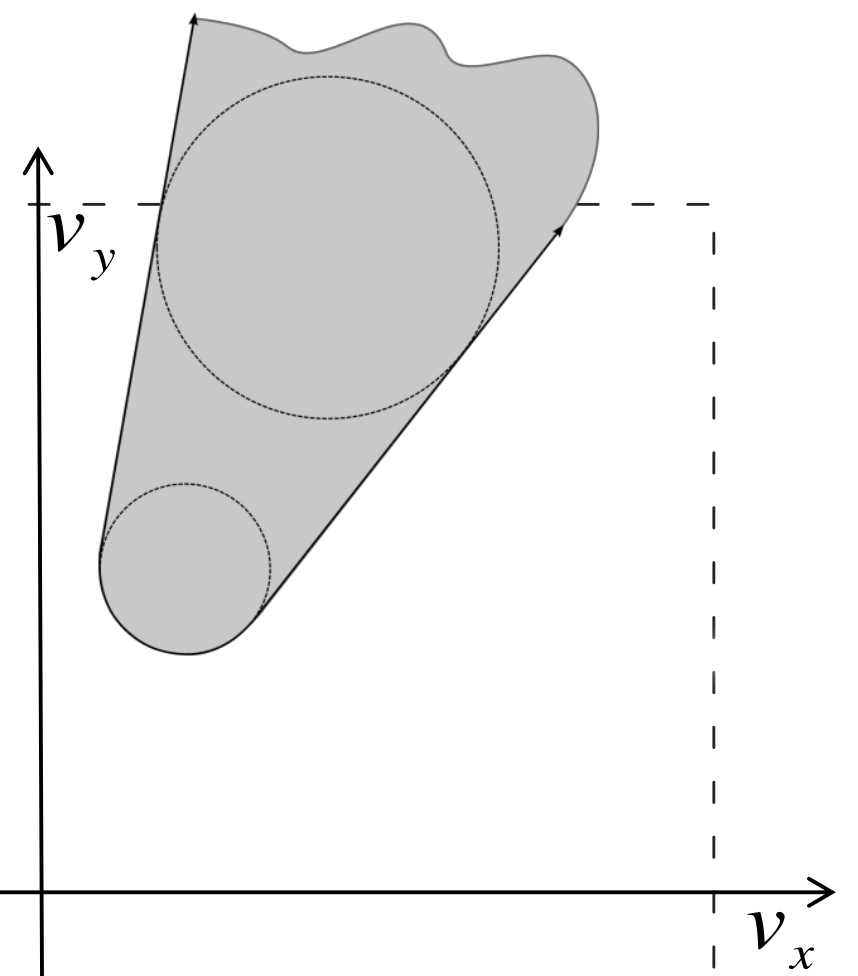
\includegraphics[width=0.97\linewidth]{./Figures/06_VO.png}
        \end{minipage}
        \begin{itemize}
            \ides{Velocity Obstacle:} Velocities in velocity space which lead to collisions in less than $\tau$ time
        \item $\text{VO}_\text{RO}^\tau = \bigcup_{0 \le t \le \tau} D(-\frac{p_\text{RO}}{t}, \frac{r_\text{RO}}{t})$
                \begin{itemize*}
                    \ides{$\mathbf{p_\text{RO}}$:} Relative position between robot and obstacle
                    \ides{$\mathbf{\text{VO}_\text{RO}}$:} Relative velocity between robot and obstacle
                    \ides{$\mathbf{r_\text{R/O}}$:} Radius of robot/obstacle
                    \ides{$\mathbf{D(x,y)}$:} Disc centred at $(x,y)$
                \end{itemize*}
            \item Multiple objects lead to multiple velocity obstacle regions
            \item Robot selects any velocity outside of the complement of VOs
            \icon Does not model interaction effects
    \end{itemize}
    \ides{Reciprocal Velocity Obstacles (RVO)}
        \begin{minipage}[b]{0.5\linewidth}
            \raggedright
            \begin{itemize}
                \item Assume:
                    \begin{itemize*}
                        \item Robot moves on piece-wise linear curves
                        \item Robot is omnidirectional
                        \item Robot and obstacles are circular
                        \item Fair behaviour of all agents
                    \end{itemize*}
            \item Identical to CO, but collision avoidance is shared between interaction agents
            \end{itemize}
        \end{minipage}
        \begin{minipage}[b]{0.45\linewidth}
            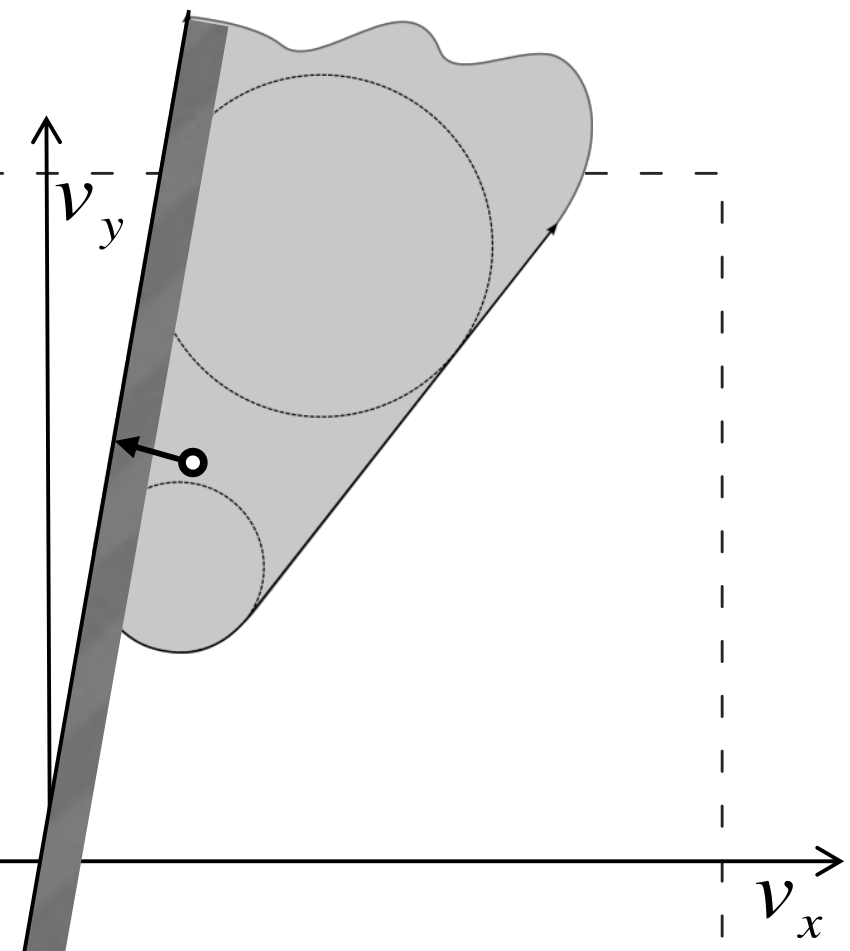
\includegraphics[width=\linewidth]{./Figures/06_RVO.png}
        \end{minipage}
        \begin{itemize}
            \item Operate in relative velocity space
            \item Linear constraints decides if obstacles are avoided to the left or right
                \begin{itemize}
                    \item Tangent to the boundary of the CO which is closer to the current velocity
                \end{itemize}
            \ides{Current relative velocity leads to collision:} Shift at least with half the velocity difference to the linear constraint
            \ides{Current relative velocity does not lead to collision:} Shift at most with half the velocity difference towards the linear constraint
        \end{itemize}
\end{itemize}
